\section{Training Data Generation}
\label{section:data_generation}

Our goal is to study whether such legal reasoning KGs would benefit LLMs on diverse tasks by conducting both SFT and Preference Optimization. In this section, we present how we utilized our IRAC KG to produce the corresponding training data.

\begin{figure*}[ht]
  \center
  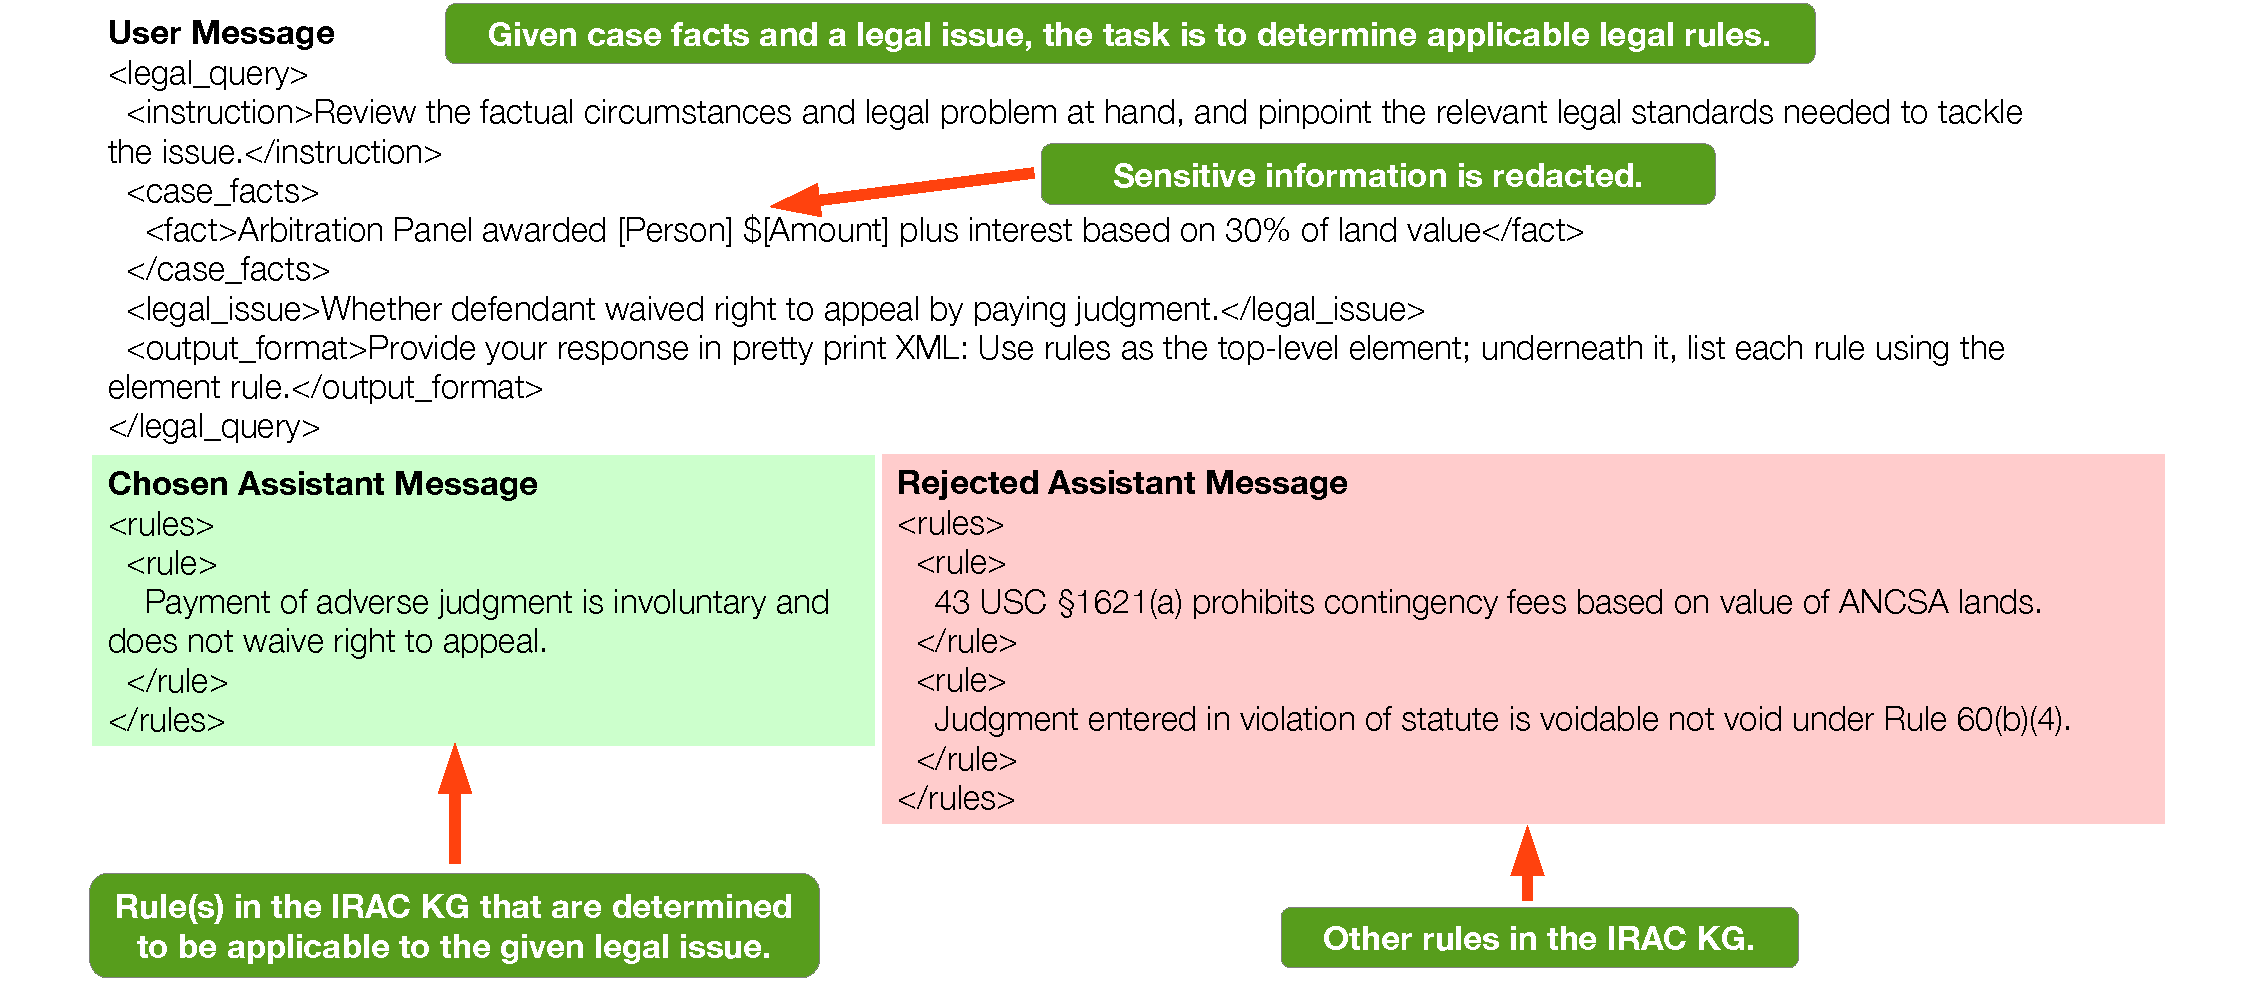
\includegraphics[width=1.0\linewidth]{figure/rules_dpo}
  \caption{An example of the Rules preference dataset.}
  \label{figure:rules_dpo}
\end{figure*}

\subsection{The Rules SFT Dataset}
\label{section:rules_sft}

Figure \ref{figure:rules_sft} illustrates a concrete example of our SFT dataset. The core idea is to simulate how courts identify rule(s) that are applicable to addressing a specific legal issue. In SFT input, the main component is \textit{case\_facts}, which is the foundation to have a legal case. Then, in the training target, we teach a model how to derive the legal issue that arises from the fact(s), and further identify the applicable rule(s). In addition, we also provide an explanation on why the rule(s) are applicable to the legal issue.

Algorithm \ref{algorithm:rules_sft} depicts this SFT data generation process.
\begin{algorithm}[ht]
\caption{GenSFT($KG, l_{i}, LLM$), $KG$ represents the IRAC KG; $l_{i}$ denotes a legal issue in $KG$; a large language model $LLM$ produces an explanation on the applicability of certain rule(s) to $l_{i}$.}
\label{algorithm:rules_sft}

\begin{algorithmic}[1]
\State{$Rules \gets \emptyset$}
\State{$Facts \gets GetRelatedFacts(KG, l_{i})$}
\ForAll {$f \in Facts$}
	\State{$R_{f} \gets GetRsViaApply(KG, f)$}
	\State{$Rules \gets Rules \cup R_{f}$}
\EndFor
\State{$OtherRs \gets GetRsViaAddress(KG, l_{i})$}
\State{$Rules \gets Rules \cup OtherRs$}
%\State{$Facts, Rules \gets GetFactsRules(KG, l_{i})$}
\State{$Exp \gets Explain(LLM, l_{i}, Rules, Facts)$}
\State{\Return {$Facts, Rules, Exp$}}
\end{algorithmic}
\end{algorithm}
At Line 2, $Facts$ consists of all facts related to legal issue $l_{i}$, via the \textit{\textbf{arise from}} relation in Figure \ref{figure:kg_schema}. Next, from Line 3 to 8, we find the set of applicable rules to $l_{i}$ both directly and indirectly. On one hand, at Line 4, for each fact $f$ related to $l_{i}$, Function $GetRsViaApply(KG, f)$ finds the rules that were applied to $f$ by following the path: \textit{Rules$ \rightarrow$ \textbf{apply} $\rightarrow$ Facts}. On the other hand, at Line 7, by following the \textit{Rules $\rightarrow$ \textbf{address} $\rightarrow$ Legal Issues} chain in Figure \ref{figure:kg_schema}, Function $GetRsViaAddress(KG, l_{i})$ gathers additional rules identified by the court that could be used to address $l_{i}$ but may not actually be applied to any facts, e.g., rules from similar precedents.
%At Line 1, for legal issue $l_{i}$, we retrieve all its related facts and rules in the $KG$ (defined in Algorithm \ref{algorithm:facts_rules_for_issue}). 
As demonstrated in Figure \ref{figure:rules_sft}, the retrieved facts become SFT input, while the rules and the legal issue itself are part of the training target.

In addition, at Line 9, we prompt (Appendix \ref{section:appendix_prompt_sft}) an LLM to produce a concise explanation on why the rules are applicable to the legal issue $l_{i}$, hoping to provide more legal knowledge to downstream training tasks; this explanation constitutes another section of the training target. We conducted a quality review of 15 SFT examples with three subject matter experts (SMEs), where each example was labeled by a single SME. Among these, 11, 4 and 0 examples were graded as \textit{Correct}, \textit{Correct with minor issues} and \textit{Wrong} respectively, verifying the quality of our SFT dataset.

%We define the sub-routine $GetFactsRules$ in Algorithm \ref{algorithm:facts_rules_for_issue}.
%\begin{algorithm}[ht]
%\caption{GetFactsRules($KG, l_{i}$), $KG$ represents the IRAC KG; $l_{i}$ denotes a legal issue in the $KG$; returns all relevant $Facts$ and $Rules$ to $l_{i}$.}
%\label{algorithm:facts_rules_for_issue}

%\begin{algorithmic}[1]
%\State{$Rules \gets \emptyset$}
%\State{$Facts \gets GetRelatedFacts(KG, l_{i})$}
%\ForAll {$f \in Facts$}
%	\State{$R_{f} \gets GetRsViaApply(KG, f)$}
%	\State{$Rules \gets Rules \cup R_{f}$}
%\EndFor
%\State{$OtherRs \gets GetRsViaAddress(KG, l_{i})$}
%\State{$Rules \gets Rules \cup OtherRs$}
%\State{\Return {$Facts, Rules$}}
%\end{algorithmic}
%\end{algorithm}
%At Line 2, $Facts$ consists of all facts related to legal issue $l_{i}$, via the \textit{arises from} relation (Figure \ref{figure:kg_schema}). Next, from Line 3 to 7, we find the set of applicable rules to $l_{i}$ both directly and indirectly. On one hand, for each fact $f$ related to $l_{i}$, we find the rules that are directly connected to $f$ via the \textit{apply} relation. On the other hand, at Line 7, via the \textit{address} relation, we gather additional rules identified by the court that could be used to address the issue but may not actually be applied to any facts, e.g., rules from similar precedents.

\begin{table*}[ht]
  \centering
  \begin{tabular}{l|cccc|cccc}
    \hline
   \multirow{2}{*}{\textbf{Entity}} & \multicolumn{4}{c|}{\textbf{Claude Sonnet 3.5 KG}} & \multicolumn{4}{c}{\textbf{Llama-3.1-405B-Instruct KG}} \\
    & \textbf{Good} & \textbf{Acceptable} & \textbf{Poor} & \textbf{M} & \textbf{Good} & \textbf{Acceptable} & \textbf{Poor} & \textbf{M} \\
    \hline
    Fact & 68\% & 5\% & 2\% & 26\% & 50\% & 9\% & 6\% & 35\% \\ \hline
    Legal Issue & 63\% & 0\% & 0\% & 37\% & 75\% & 5\% & 10\% & 10\% \\ \hline
    Rule & 69\% & 0\% & 4\% & 27\% & 29\% & 0\%& 33\% & 38\% \\ \hline
    Conclusion & 68\% & 0\% & 0\% & 32\% & 60\% & 0\% & 10\% & 30\% \\ \hline \hline
    \multirow{2}{*}{\textbf{Relation}} & \multicolumn{2}{c}{\textbf{Pass}} & \multicolumn{2}{c|}{\textbf{Fail}} & \multicolumn{2}{c}{\textbf{Pass}} & \multicolumn{2}{c}{\textbf{Fail}} \\
    & \multicolumn{2}{c}{92\%} & \multicolumn{2}{c|}{8\%} & \multicolumn{2}{c}{59\%} & \multicolumn{2}{c}{41\%} \\ \hline
  \end{tabular}
  \caption{\label{table:kg_quality_review}
    IRAC KG quality review. \textit{Fact}, \textit{Legal Issue}, \textit{Rule} and \textit{Conclusion} correspond to the entity types in our IRAC KG in Figure \ref{figure:kg_schema}; we report a single number for all relations. For entities, our SMEs labeled them as \textbf{\textit{Good}} (high-quality with potentially minor inaccuracies), \textbf{\textit{Acceptable}} (with noticeable issues but still useful) and \textbf{\textit{Poor}} (with significant errors or completely incorrect); our SMEs also checked whether the KG missed any entities (\textbf{\textit{M}}) by reading the entire case. As for relations, our review only examines whether they are correct or not. Note that if any of the entities involved in a relation is judged as \textbf{\textit{Poor}}, then this relation will be labeled as \textbf{\textit{Fail}}. We determined these quality review criteria together with our domain experts.
  }
\end{table*}

\subsection{The Rules Preference Dataset}
\label{section:rules_dpo}

In addition to SFT, we also performed Preference Optimization in this work. Similar to the SFT dataset, we produced our preference data by utilizing the IRAC KG with a focus on teaching the models to correctly identify the proper legal rules to cope with a given legal issue. Figure \ref{figure:rules_dpo} shows a concrete example of this dataset. Different from the above SFT data, our preference training input (i.e., \textit{User Message}) includes both \textit{case\_facts} and \textit{legal\_issue}, with chosen and rejected legal rules as the training target. Our hypothesis is that by teaching models how to select the appropriate rules for different legal matters, they would be able to gain more knowledge on how courts reason in a variety of legal situations.

We formally present the data generation process in Algorithm \ref{algorithm:rules_dpo}.
\begin{algorithm}[ht]
\caption{GenPref($KG, l_{i}, LJ$), $KG$ denotes the IRAC KG; $l_{i}$ is a legal issue in $KG$; an LLM Judge $LJ$ determines a rule's applicability to $l_{i}$.}
\label{algorithm:rules_dpo}

\begin{algorithmic}[1]
\State{$Facts \gets GetRelatedFacts(KG, l_{i})$}
\State{$Chosen\_Rs \gets \emptyset$}
\ForAll {$f \in Facts$}
	\State{$R_{f} \gets GetRsViaApply(KG, f)$}
	\State{$Chosen\_Rs \gets Chosen\_Rs \cup R_{f}$}
\EndFor
\State{$OtherRs \gets GetRsViaAddress(KG, l_{i})$}
\State{$Chosen\_Rs \gets Chosen\_Rs \cup OtherRs$}
%\State $Fs, Chosen\_Rs \gets GetFactsRules(KG, l_{i})$
\State $Rejected\_Rs \gets All\_Rs \setminus Chosen\_Rs$
\ForAll {$r \in Rejected\_Rs$}
	\If {$Applicable(LJ, Facts, l_{i}, r)$}
		\State {$Rejected\_Rs \gets Rejected\_Rs \setminus \{r\}$}
	\EndIf
\EndFor
\State {\Return {$Facts, Chosen\_Rs, Rejected\_Rs$}}
\end{algorithmic}
\end{algorithm}
For preference training, we need to provide both the chosen and the rejected rules. Similar to SFT data generation, at Line 1, we first obtain facts ($Facts$) related to the legal issue $l_{i}$. Then, from Line 2 to 8, we find the chosen rules ($Chosen\_Rs$) that are either directly (via the \textit{\textbf{address}} relation) or indirectly (via the combination of the \textit{\textbf{apply}} and the \textit{\textbf{arise from}} relations) connected to $l_{i}$. In order to produce the rejected rules, from Line 9 to 14, we use an LLM judge (Appendix \ref{section:appendix_prompt_dpo}) to determine whether each of the non-chosen rules is truly not applicable. The intuition is that even though a rule is not directly or indirectly connected to $l_{i}$ in the KG, it may be due to an imperfect KG generation process. The output of the LLM Judge could be: \textit{Yes}/\textit{No}/\textit{Potentially}, and we only keep the rules that are determined as non-applicable (i.e., the LLM Judge outputs \textit{No}).

\subsection{Model Training}
\label{section:model_training}

In our work, we conduct both SFT and Preference Optimization, DPO \cite{DBLP:conf/nips/RafailovSMMEF23} specifically. By giving models the case facts, SFT (Figure \ref{figure:rules_sft}) teaches the models how to identify the legal issue, locate the applicable rules, and learn the rationale behind these materials (\textit{Exp} at Line 9 in Algorithm \ref{algorithm:rules_sft}). Different from SFT, our preference data (Figure \ref{figure:rules_dpo}) focuses on teaching the models how to conduct legal reasoning by contrasting the applicable and non-applicable legal rules with respect to a variety of legal matters. For DPO, we adopted the default Loss function with a small NLL term on the chosen answers \cite{DBLP:journals/corr/abs-2404-19733}.
%\begin{equation}
%  \label{equation:dpo}
%  Loss = Loss_{dpo} + \alpha Loss_{nll}
%\end{equation}
%where $\alpha$ controls how much weight we give to the NLL loss on the chosen answers.

We emphasize that the above training data is not directly related to our evaluation benchmarks (Section \ref{section:evaluation_benchmarks}). Our primary goal is to provide the models with high-quality domain knowledge via different training paradigms in order to study whether the trained models would be able to gain improved capability on diverse tasks in the same domain.
